\section{validity confirmation through the Union Bound}
\label{sec4}
%For a given RSC code, the distance spectrum provides information concerning the multiplicity of a codeword for a fixed weight and it is an effective tool to evaluate its error-correcting capability. In practice however, since higher-weight codewords have very little effect on its overall error-correcting capability, we usually use a partial distance spectrum, where the largest codeword weight value is set to $d_{\text{max}}$. 

%The distance spectrum of the RSC code can be obtained from its transfer function, denoted by $$T(Y,X)=\sum_{d=0}^{\infty}\sum_{w=0}^{\infty} a(d,w)Y^dX^w$$ where $a(d,w)$ is the number of codewords of weight $d$ generated by an input bit sequence of weight $w$. 
%The transfer function enumerates all the paths that diverge from and then return to the initial state \cite{ref3}, \textit{i.e.} the RTZ input paths. 
%Once the transfer function of an RSC code is known, it can be used to obtain bounds on the error-correcting capability using the union bound.
%Unfortunately, the complexity involved in deriving the transfer function increases as the number of states of the RSC code increases and other methods such as Mason's Rule \cite{ref3} have to be used. 

%For a given RSC code, we have shown in \ref{subsec:low-weight} that each codeword $c(x)$ is made up of $b(x)$ and $h(x)$ which have $a(x)$ as their common factor as shown in (\ref{novelEq2}) and (\ref{novelEq3}).
 In this section, we obtain a union bound using the low-weight codeword components pattern list and,  in order to confirm the validity of our proposed method, compare it to the union bound obtained via the transfer function as well as simulation results.

\subsection{A novel union bound}
Let $\cA_h(d)$ be the set of all $a(x)$ which yields weight-$d$ PCs \ie, $w_H(h(x))=w_H(a(x)f(x))=d$ for $a(x) \in \cA_h(d)$. We also define $\cA_b(d)$ and $\cA_c(d)$ as the sets of all $a(x)$s which result weight-$d$ SCs and codewords, respectively.

Then, for $w_H(b(x)), w_H(h(x)) \geq 2$, we have from \eqref{eq:cw-weight} that
\begin{align}
\cA_c(d) = \bigcup_{\ell = 2}^{d-2} \left\{\cA_b(\ell) \cap \cA_h(d-\ell)\right\}
\label{Eq:exactset}
\end{align}
However, to determine $\cA_b(\ell)$ or $\cA_h(\ell)$ for a large $\ell$ is a complex task in general. Thus, in this paper, we replace the set $\cA_c(d)$ by the following approximated set %\eqref{setApprox}
\begin{equation}
\begin{split}
\cA_c(d) \approx \cA_c'(d) &= \left\{\bigcup_{\ell = 2}^{\ell+1} \left\{\cA_b(\ell) \cap \cA_h(d-\ell)\right\}\right\}\bigcup \left\{\bigcup_{\ell = 2}^{\ell+1} \left\{\cA_b(d-\ell) \cap \cA_h(\ell)\right\}\right\}
\end{split}
\label{setApprox}
\end{equation}
and obtain an approximated union bound as
\begin{align}
P_b \leq \frac{1}{k} \sum_{d=d_{\text{free}}}^{d_{\text{free}+1}} \sum_{a(x) \in \cA'_c(d)}w_H(a(x)g(x)) Q\Bigg( \sqrt{\frac{2dE_c}{N_0}}\Bigg)
\label{novelEq7}
\end{align}
Notice that since $\cA_c(d)$ in \eqref{Eq:exactset} is replaced by $\cA_c'(d)$, the contributions of the codewords with $\ell \approx d-\ell$ may be neglected in our approximation.

To obtain $\cA_c'(d)$, based on $f(x)$, we first generate the set consisting of $a(x)$s which yield the weight-2 and -3 PCs, \ie~$\cA_h(2)\cup\cA_h(3)$. Next, for each $a(x) \in \cA_h(2)\cup\cA_h(3)$, we determine the corresponding SC $b(x)=a(x)g(x)$. Similarly, we determine the PC $h(x)=a(x)f(x)$ for each $a(x)$ in the set $\cA_s(2)\cup\cA_s(3)$  obtained based on $g(x)$. Finally, we narrow down the corresponding codewords as $w_H(b(x))+w_H(h(x)) \leq d_{\text{free+3}}$ for $a(x) \in \cA_h(2)\cup\cA_h(3)\cup\cA_s(2)\cup\cA_s(3)$.

In order to confirm the validity of the proposed method, we evaluated {\it bit error rate} (BER) through computer simulations for the codes listed in Table \ref{TB:Codes}. For Code I, the low-weight PCs and SCs can be founed in Examples \ref{ex-3} and \ref{ex-1}, respectively, while Examples \ref{ex-2} and \ref{ex-3}, respectively, provide those of Code II.
\begin{table}[htbp]
	\caption{The generator polynomials of $5/7$, $37/21$, and $23/35$ RSC codes}
	\centering
	\begin{tabularx}{0.75\textwidth}{clll} 
		\toprule
			& Generation fuction & $f(x)$ & $g(x)$ \\ %[0.5ex] 
		\midrule
		Code I & 5/7 & $1+x^2$ (Ex. \ref{Ex:4}) & $1+x+x^2$ (Ex. \ref{Ex:1})\\
		Code II & 37/21 & $1+x+x^2+x^3+x^4$ (Ex. \ref{Ex:3})& $1+x^4$  (Ex. \ref{Ex:4})\\
		Code III & 23/35 & $1+x+x^4$ (Ex. \ref{Ex:2})& $1+x^2+x^3+x^4$  (Ex. \ref{Ex:5})\\
		\bottomrule
	\end{tabularx}
	\label{TB:Codes}
\end{table}


\begin{table}[htbp]
		\caption{SCs and PCs for Code I}
		\centering
		\begin{tabularx}{0.75\textwidth}{|c|c|XXX} 
			\toprule
			$w_H(c(x))$&~& $a(x)$ & $b(x)$ & $h(x)$ \\ %[0.5ex] 
			\midrule
			5& ~&$1$ & $1+x+x^{2}$ & $1+x^2$\\
			\cline{1-5}
			6& ~&$1+x$ & $1+x^3$ & $1+x+x^2+x^3$\\
			&~ &$1+x^2$ & $1+x+x^3+x^4$ & $1+x^{4}$\\
			&~&$1+x+x^2$ & $1+x^2+x^4$ & $1+x+x^3+x^4$\\
			&~&$1+x+x^3$ & $1+x^4+x^5$ & $1+x+x^2+x^5$\\
			\cline{1-5}
			7&~&$1+x^2+x^3$ & $1+x+x^5$ & $1+x^3+x^4+x^5$\\
			&~&$1+x^2+x^4$ & $1+x+x^3+x^5+x^6$ & $1+x^{6}$\\			
			\cline{1-5}
			&~&$1+x+x^3+x^4$ & $1+x^6$ & $1+x+x^2+$\\
			&Found&&&$x^4+x^5+x^6$\\
			&~&$1+x^2+x^4+x^6$ & $1+x+x^3+x^5+x^7+x^8$ & $1+x^8$\\
			\cline{2-5}
			8&&$1+x+x^2+x^3$ 		&$1+x+x^3+x^5$ 		& $1+x+x^4+x^5$\\
			&&$1+x+x^2+x^4$ 		&$1+x^2+x^5+x^6$		& $1+x+x^3+x^6$\\
			&Not Found&$1+x+x^3+x^5$ 		&$1+x^4+x^6+x^7$ 		& $1+x+x^2+x^7$\\
			&&$1+x^2+x^3+x^4$ 	&$1+x+x^4+x^6$ 		& $1+x^3+x^5+x^6$\\
			&&$1+x^2+x^3+x^5$ 	&$1+x+x^6+x^7$ 		& $1+x^3+x^4+x^7$\\
			&&$1+x^2+x^4+x^5$ 	&$1+x+x^3+x^7$ 		& $1+x+x^6+x^7$\\
			\bottomrule
		\end{tabularx}		
		\label{code-tables-1}
	\end{table}


\begin{table}[htbp]
		\caption{SCs and PCs for Code II}
		\centering
		\begin{tabularx}{0.75\textwidth}{|c|c|XXX} 
			\toprule
			$w_H(c(x))$&~& $a(x)$ & $b(x)$ & $h(x)$ \\ %[0.5ex] 
			\midrule
			6&~&$1+x$ & $1+x+x^{4}+x^5$ & $1+x^5$\\
			\cline{2-5}
			7&~&$1$ & $1+x^4$ & $1+x+x^2+x^3+x^4$\\
			\cline{1-5}
			&Found&$1+x+x^5+x^6$ & $1+x+x^4+x^6+x^9+x^{10}$ & $1+x^{10}$\\
			\cline{2-5}
			8&Not Found&$1+x^2$ 				&$1+x^2+x^4+x^6$ 		& $1+x+x^5+x^6$\\
			&~&$1+x+x^4+x^6$ 		&$1+x+x^8+x^9$			& $1+x^4+x^5+x^9$\\
			\cline{1-5}
			&&$1+x+x^4$ 		&$1+x+x^5+x^8$ 		& $1+x^4+x^6+x^7+x^8$\\
			&&$1+x^2+x^4$ 		&$1+x^2+x^6+x^8$ 		& $1+x+x^4+x^7+x^8$\\
			9&Not Found&$1+x^3+x^4$ 	&$1+x^3+x^7+x^8$ 		& $1+x+x^2+x^4+x^8$\\
			&&$1+x+x^5$ 		&$1+x+x^4+x^9$ 		& $1+x^6+x^7+x^8+x^9$\\
			&&$1+x^4+x^5$ 		&$1+x^5+x^8+x^9$ 		& $1+x+x^2+x^3+x^9$\\
			\bottomrule
		\end{tabularx}		
		\label{code-tables-2}
	\end{table}


	\begin{table}[htbp]
		\caption{SCs and PCs for Code III}
		\centering
		\begin{tabularx}{0.85\textwidth}{|c|c|XXX} 
			\toprule
			$w_H(c(x))$&~& $a(x)$ & $b(x)$ & $h(x)$ \\ %[0.5ex] 
			\midrule
			7&~&$1$ & $1+x^2+x^3+x^4$ & $1+x+x^{4}$\\
			  &~&$1+x^2+x^3$ & $1+x^7$ & $1+x+x^2+x^6+x^7$\\
			\cline{1-5}
			&&$1+x$ 						& $1+x+x^2+x^5$ 			& $1+x^2+x^4+x^5$\\
			8&Not Found&$1+x+x^2+x^4$ 				& $1+x+x^7+x^8$ 			& $1+x^3+x^6+x^8$\\
			&&$1+x+x^2+x^4+x^6+x^7$ 	& $1+x+x^6+x^{11}$ 			& $1+x^3+x^{10}+x^{11}$\\
			\cline{1-5}
			&~&$1+x+x^2+x^3+x^5$ & $1+x+x^3+x^4+x^8+x^9$ & $1+x^7+x^9$\\
			9&Found&$1+x+x^2+x^3+x^5+x^7+x^8$ & $1+x+x^3+x^4+x^7+x^{12}$ & $1+x^{11}+x^{12}$\\
			\cline{2-5}
			 ~&~&$1+x+x^2$ 					& $1+x+x^4+x^6$ 			& $1+x^{3}+x^{4}+x^5+x^6$\\
			&Not Found&$1+x+x^2+x^4+x^5$ 		& $1+x+x^5+x^9$ 			& $1+x^{3}+x^{5}+x^8+x^9$\\
			\cline{1-5}
			&Found&$1+x^2+x^3+x^7+x^9+x^{10}$ & $1+x^{14}$ & $1+x+x^2+x^6+x^8+x^9+x^{13}+x^{14}$\\
						\cline{2-5}
			&&$1+x^2$ 								& $1+x^3+x^5+x^6$ 					& $1+x+x^2+x^{3}+x^{4}+x^6$\\
			&&$1+x+x^3$ 								& $1+x+x^2+x^4+x^5+x^6+x^7$ 	& $1+x+x^{3}+x^{7}$\\
			&&$1+x+x^2+x^3$ 				& $1+x+x^3+x^4+x^5+x^7$ 			& $1+x^{5}+x^6+x^7$\\
			&&$1+x^4$ 								& $1+x^2+x^3+x^6+x^7+x^8$ 		& $1+x+x^{5}+x^8$\\
			&&$1+x^2+x^3+x^5$ 						& $1+x^5+x^8+x^9$ 					& $1+x+x^{2}+x^5+x^7+x^9$\\
			&~&$1+x^2+x^4+x^5$ 						& $1+x^3+x^4+x^9$ 					& $1+x+x^{2}+x^3+x^8+x^9$\\
			10&Not Found&$1+x^2+x^3+x^6$ 						& $1+x^6+x^7+x^8+x^9+x^{10}$ 	& $1+x+x^2+x^{10}$\\
			&&$1+x+x^2+x^3+x^4+x^6$ 				& $1+x+x^3+x^5+x^9+x^{10}$ 		& $1+x^4+x^8+x^{10}$\\
			&&$1+x^3+x^5+x^6$ 						& $1+x^2+x^4+x^{10}$ 				& $1+x+x^{3}+x^{5}+x^9+x^{10}$\\
			&&$1+x+x^2+x^3+x^5+x^6$ 				& $1+x+x^3+x^4+x^6+x^{10}$ 		& $1+x^{6}+x^{9}+x^{10}$\\
			&&$1+x^2+x^3+x^7$ 						& $1+x^9+x^{10}+x^{11}$ 			& $1+x+x^{2}+x^{6}+x^8+x^{11}$\\
			&&$1+x^4+x^6+x^7$ 						& $1+x^2+x^3+x^{11}$ 				& $1+x+x^{5}+x^6+x^{10}+x^{11}$\\
			&&$1+x^2+x^3+x^5+x^7+x^8$ 			& $1+x^5+x^7+x^{12}$ 				& $1+x+x^{2}+x^5+x^{11}+x^{12}$\\
			&&$1+x^2+x^3+x^6+x^8+x^9$ 			& $1+x^6+x^7+x^{13}$ 				& $1+x+x^2+x^8+x^{12}+x^{13}$\\
			&&$1+x+x^2+x^3+x^4+x^6+x^8+x^9$ 	& $1+x+x^3+x^5+x^8+x^{13}$ 		& $1+x^{4}+x^{12}+x^{13}$\\
			\bottomrule
		\end{tabularx}		
		\label{code-tables-3}
	\end{table}






\subsection{Numerical results}
We verify the validity of our proposed method for the $5/7,~37/21$ and $23/35$ RSC codes, assuming a frame size of $N=64$ is used to obtain the simulation results. 
%, we compared the bounds in \eqref{novelEq7} with that obtained using the transfer function method as well as the simulation results for the 
%For each RSC code and a frame size of $N=64$, the codeword is BPSK modulated and transmitted over the AWGN channel. At the receiver end, the Viterbi algorithm is used to decode before a decision is made on the decoded sequence.



From Table \ref{novelTab13}, we observe that every SC such that $w_H(b(x)) >3$ is either a combination of only weight-2 SCs or only weight-3 SCs or both. This means that when the 5/7 RSC code is used in a TC, the deterministic interleaver should be designed in such a way that it deals effectively with both weight-2 and weight-3 SCs. While, having to consider weight-3 SCs in the deterministic interleaver design introduces a bit of complexity, it is manageable since there is just a single $(m,n)$ pair that is associated with the weight-3 SCs.

\begin{figure}[htbp]
	\centering
	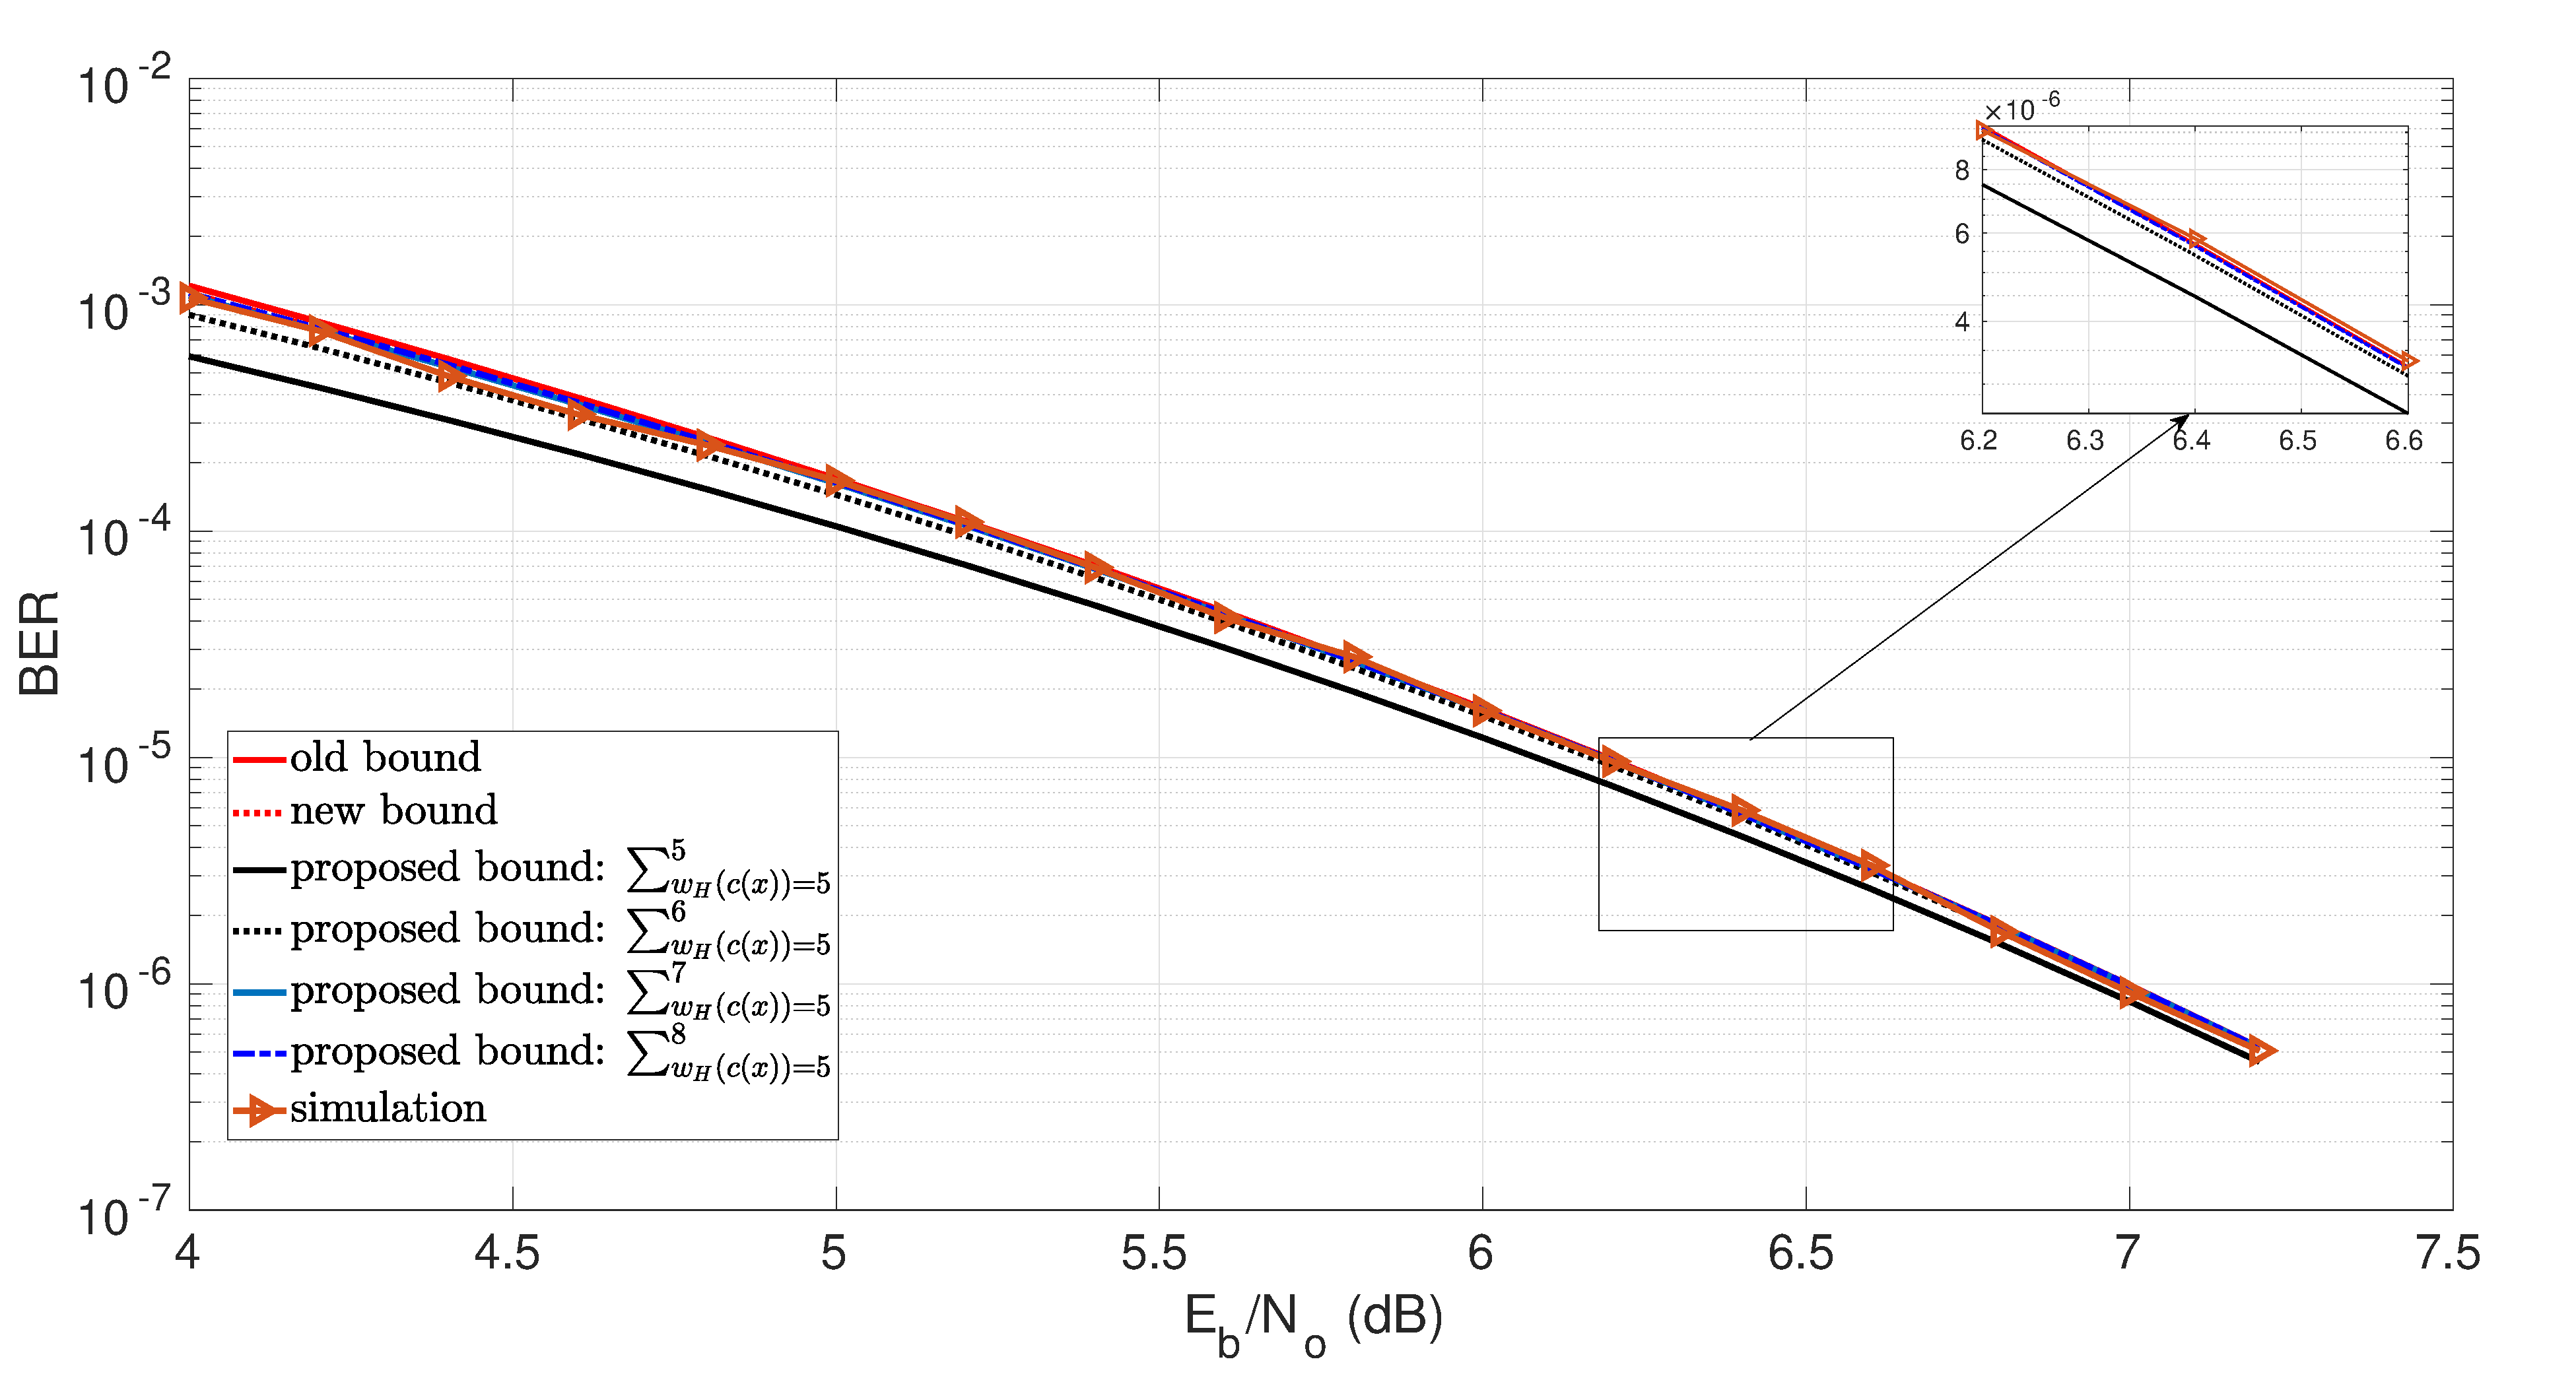
\includegraphics[width=0.5\textwidth]{./Images/RSC_5_7_lower_weights3.eps}
	\captionof{figure}{Old Bound vs New Bound vs Simulation for 5/7 RSC Code}
	\label{simFig1}
\end{figure}

Fig. \ref{simFig1} shows the simulation results for the $5/7$ RSC code as well as the union bound obtained using the transfer function and our proposed method. We can observe that the accuracy of our proposed bound increases with the number of terms used in the approximation. Also, as $E_b/N_0$ increases, the proposed bound as well as the transfer function bound and the simulation results tend to converge. The fact that just a single $(m,n)$ pair needs to be considered for weight-3 SCs during interleaver design makes the 5/7 RSC code attractive for use in TCs.
\label{ex-6}


Table \ref{novelTab14} confirms the non-existence of weight-3 SCs and PCs in the 37/21RSC code, and that every SC such that $w_H(b(x)) > 2$ is a combination of weight-2 SCs. As such, deterministic interleaver design for this RSC code is relatively simpler, since only weight-2 SCs need to be considered.
\begin{figure}[htbp]
	\centering
	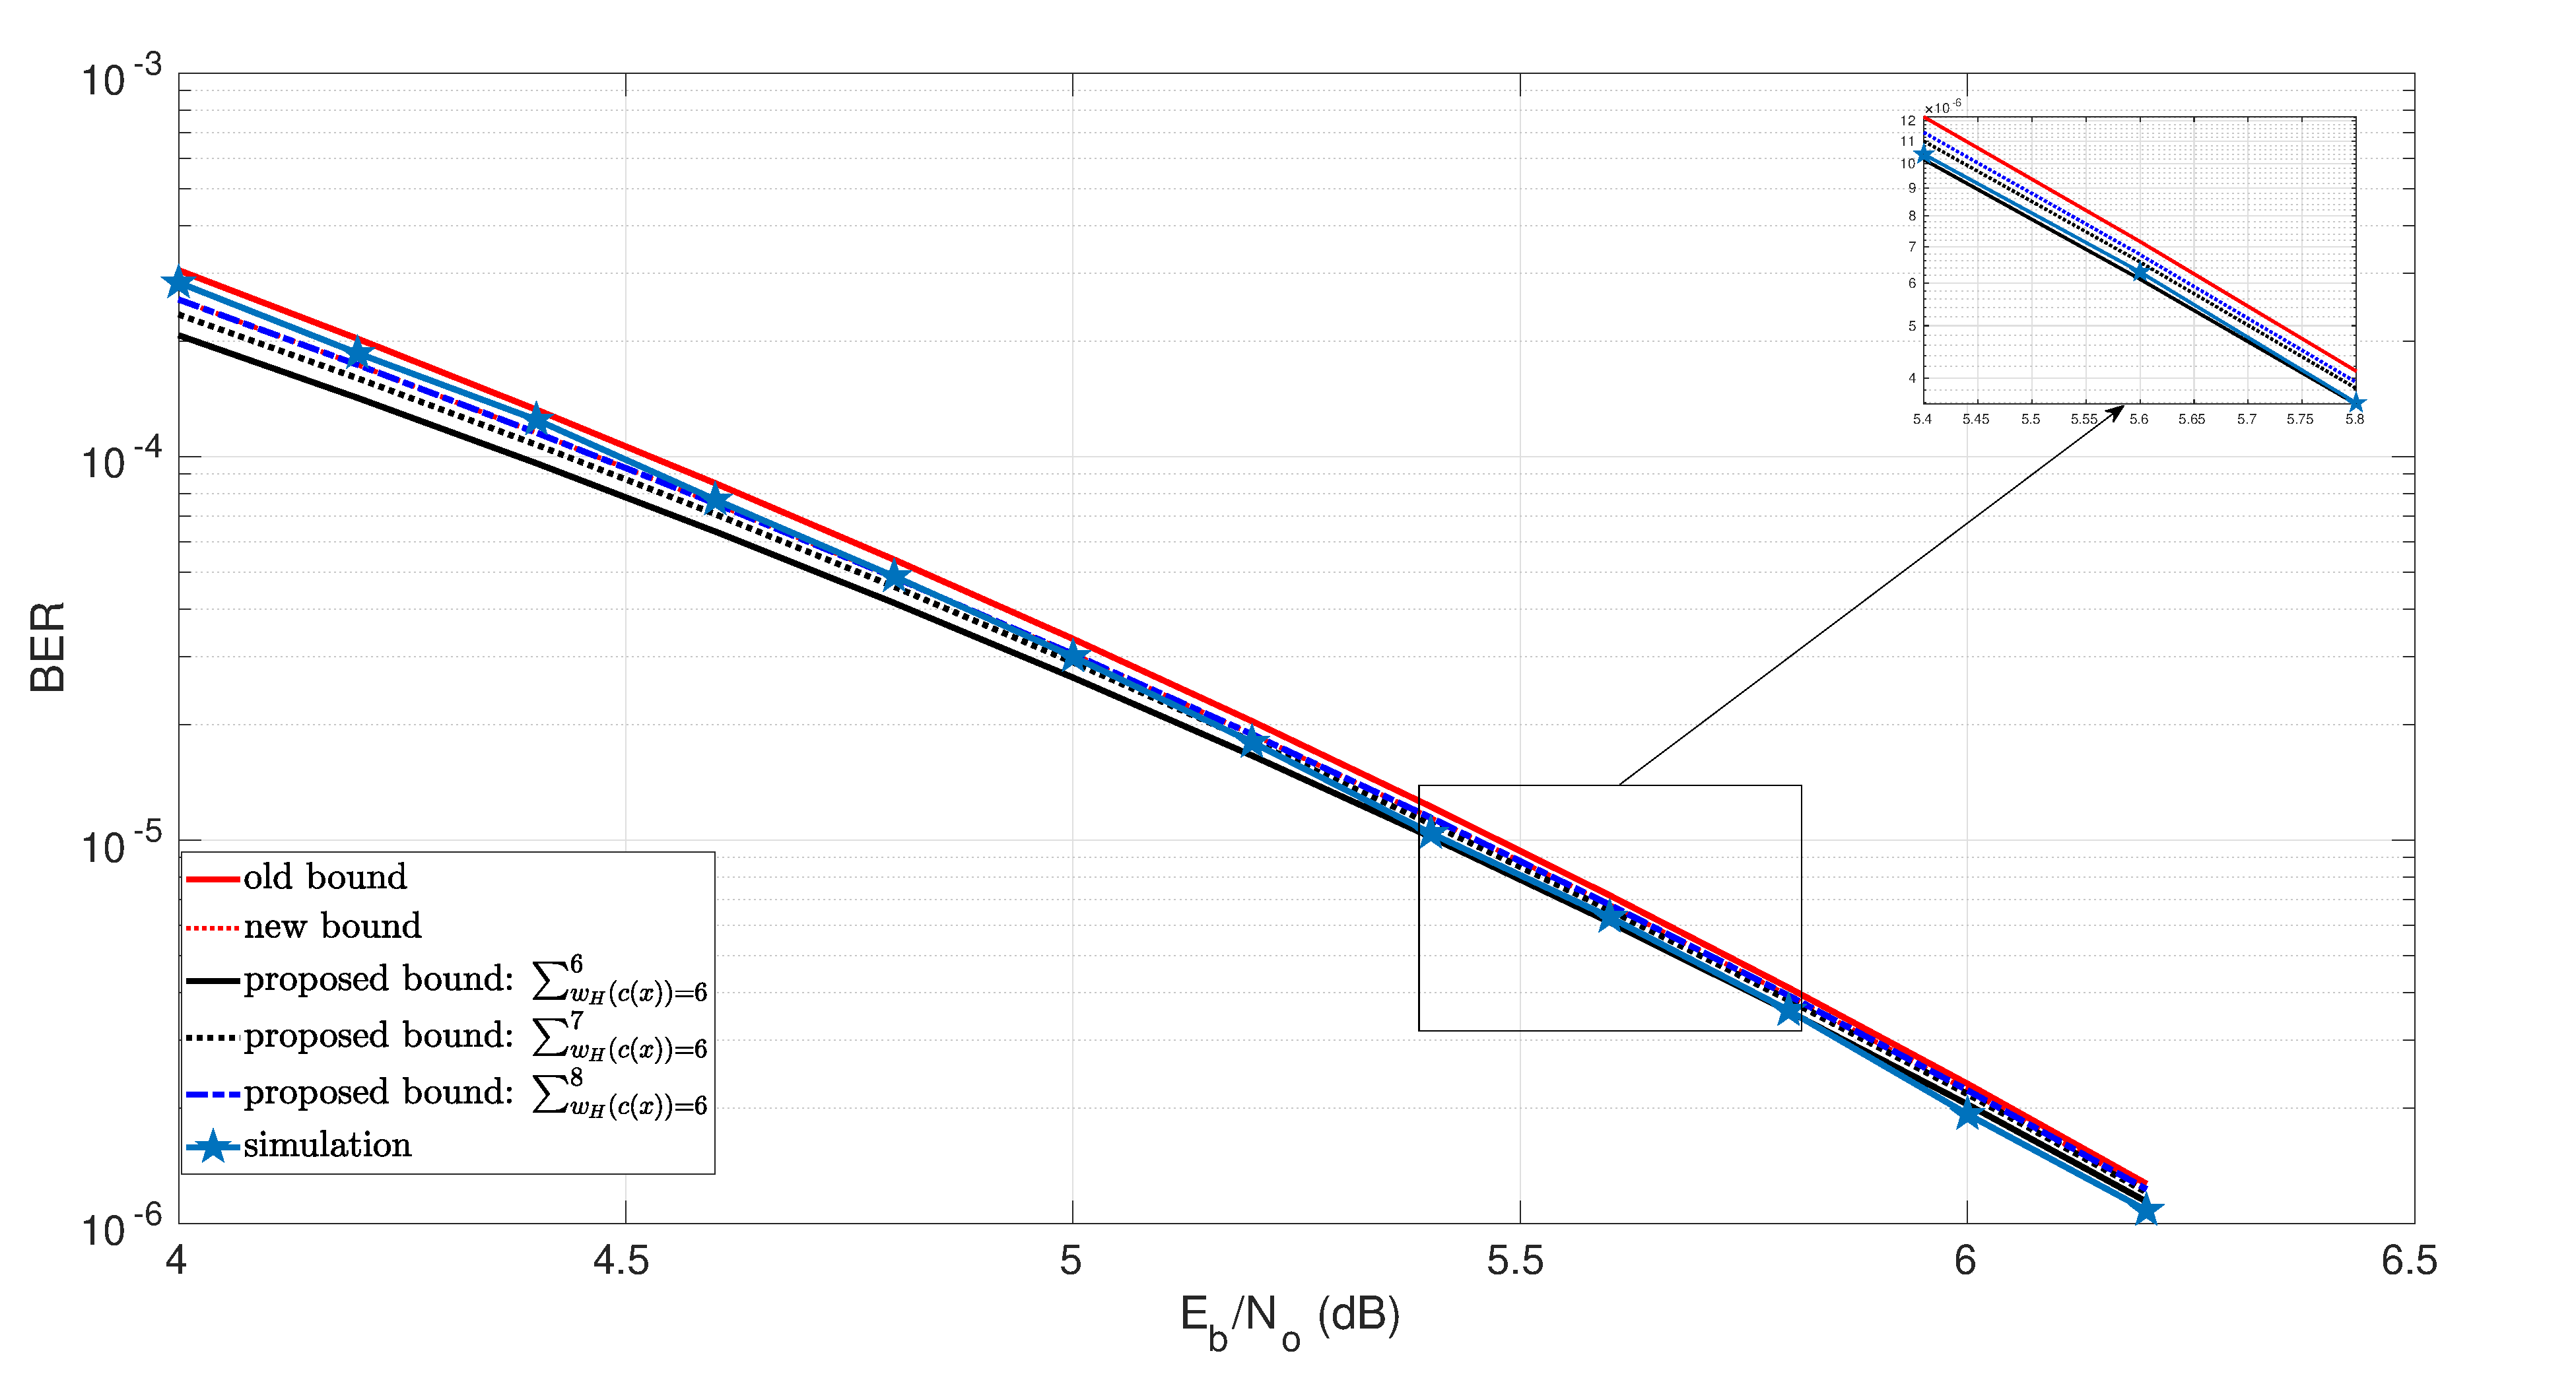
\includegraphics[width=0.5\textwidth]{./Images/RSC_37_21_lower_weights3.eps}
	\caption{Old Bound vs New Bound vs Simulation for 37/21 RSC Code}
	\label{simFig2}
\end{figure}

Simulation results, the transfer function bound and our proposed bound are shown in Fig. \ref{simFig2} for the $37/21$ RSC code. By observation, we can draw conclusions similar to  Example \ref{ex-6} with respect to the accuracy of our proposed bound . Given that weight-2 SCs and PCs are sufficient to derive the union bound, and deterministic interleaver design requires focusing on weight-2 SCs only, this RSC code is highly recommended for use in TCs.

From Table \ref{novelTab15}, we observe that there are no weight-3 SCs. However, there exists weight-4 SCs that are not a combination of weight-2 SCs and when this RSC code is used in TCs, the deterministic interleaver needs to be designed to cater for weight-2 SCs as well as such weight-4 SCs. 
 
\begin{figure}[htbp]
	\centering
	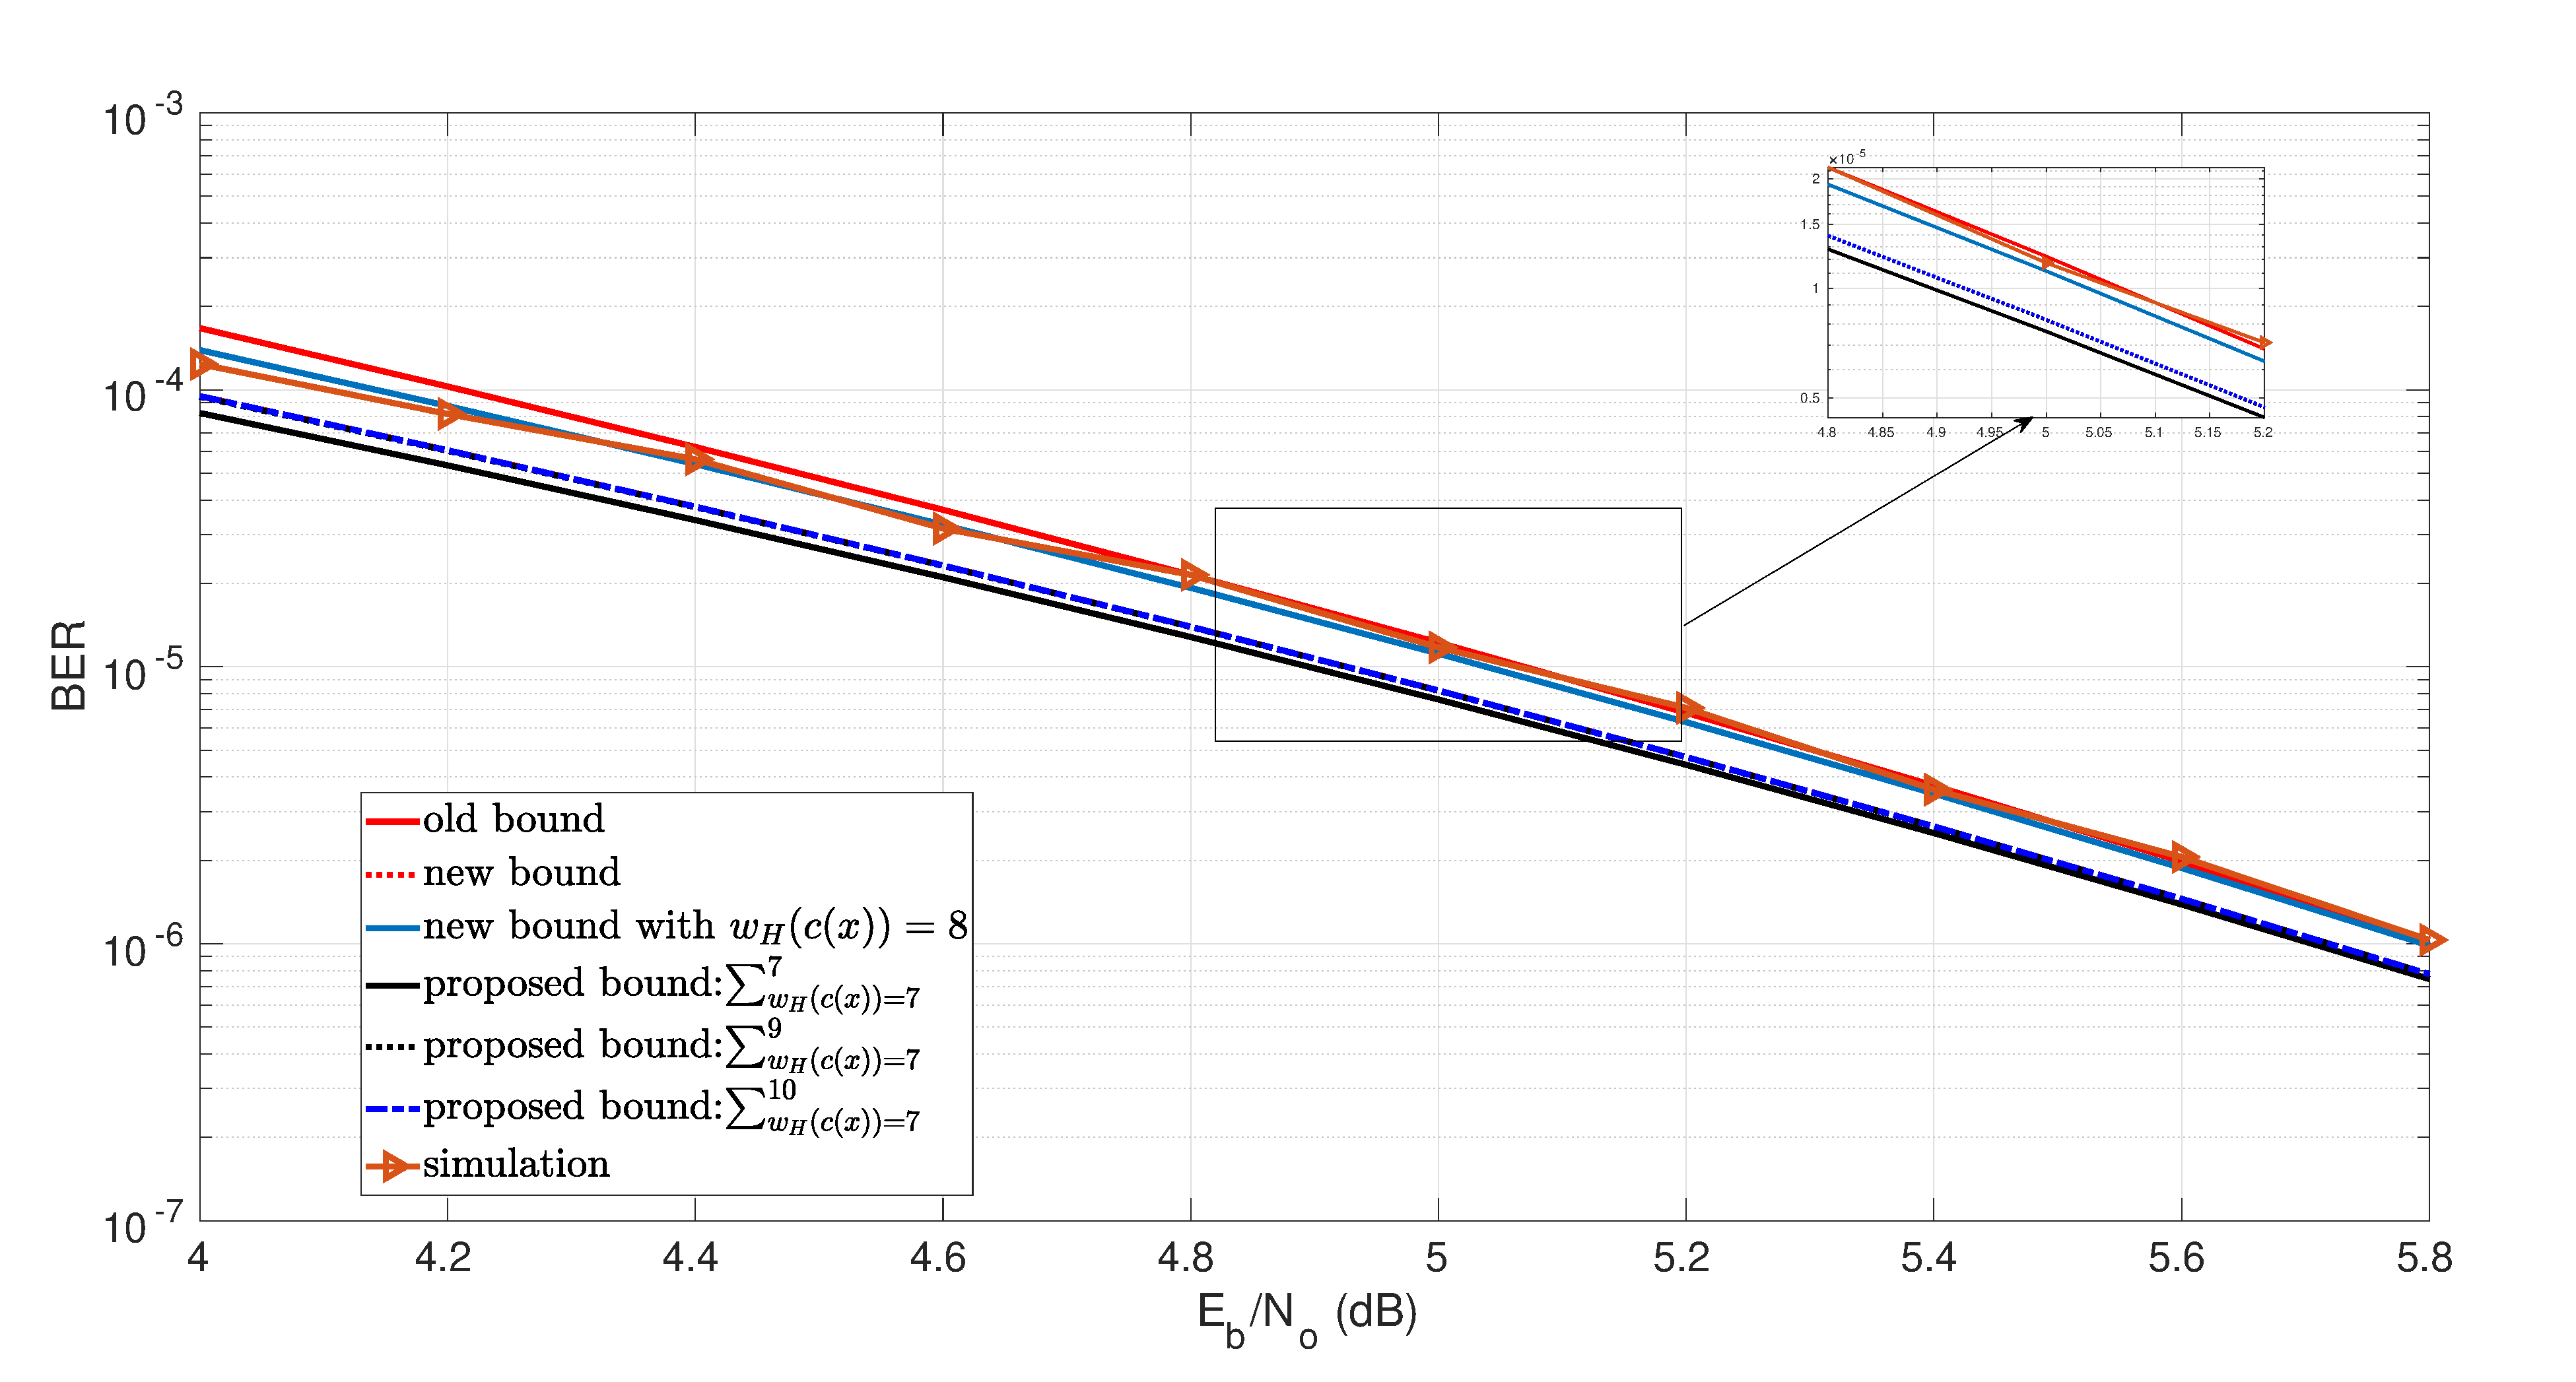
\includegraphics[width=0.5\textwidth]{./Images/RSC_23_35_lower_weights3.eps}
	\caption{Old Bound vs New Bound vs Simulation for 23/35 RSC Code}
	\label{simFig3}
\end{figure}
Fig. \ref{simFig3} shows the simulation results for the $23/35$ RSC code as well as the union bounds obtained using the transfer function as well as our proposed method. Even though the accuracy of our proposed bound increases with the number of terms use, it neither converges with the transfer function bound nor the simulation results as $E_b/N_0$ increases. Even though it is possible to improve the accuracy of our proposed bound by considering SCs and PCs of weight-4, the added complexity as a result of considering weight-4 SCs in the interleaver design process makes this RSC code very unattractive for use in TCs. 


%\begin{figure}[h!]
%\centering
%		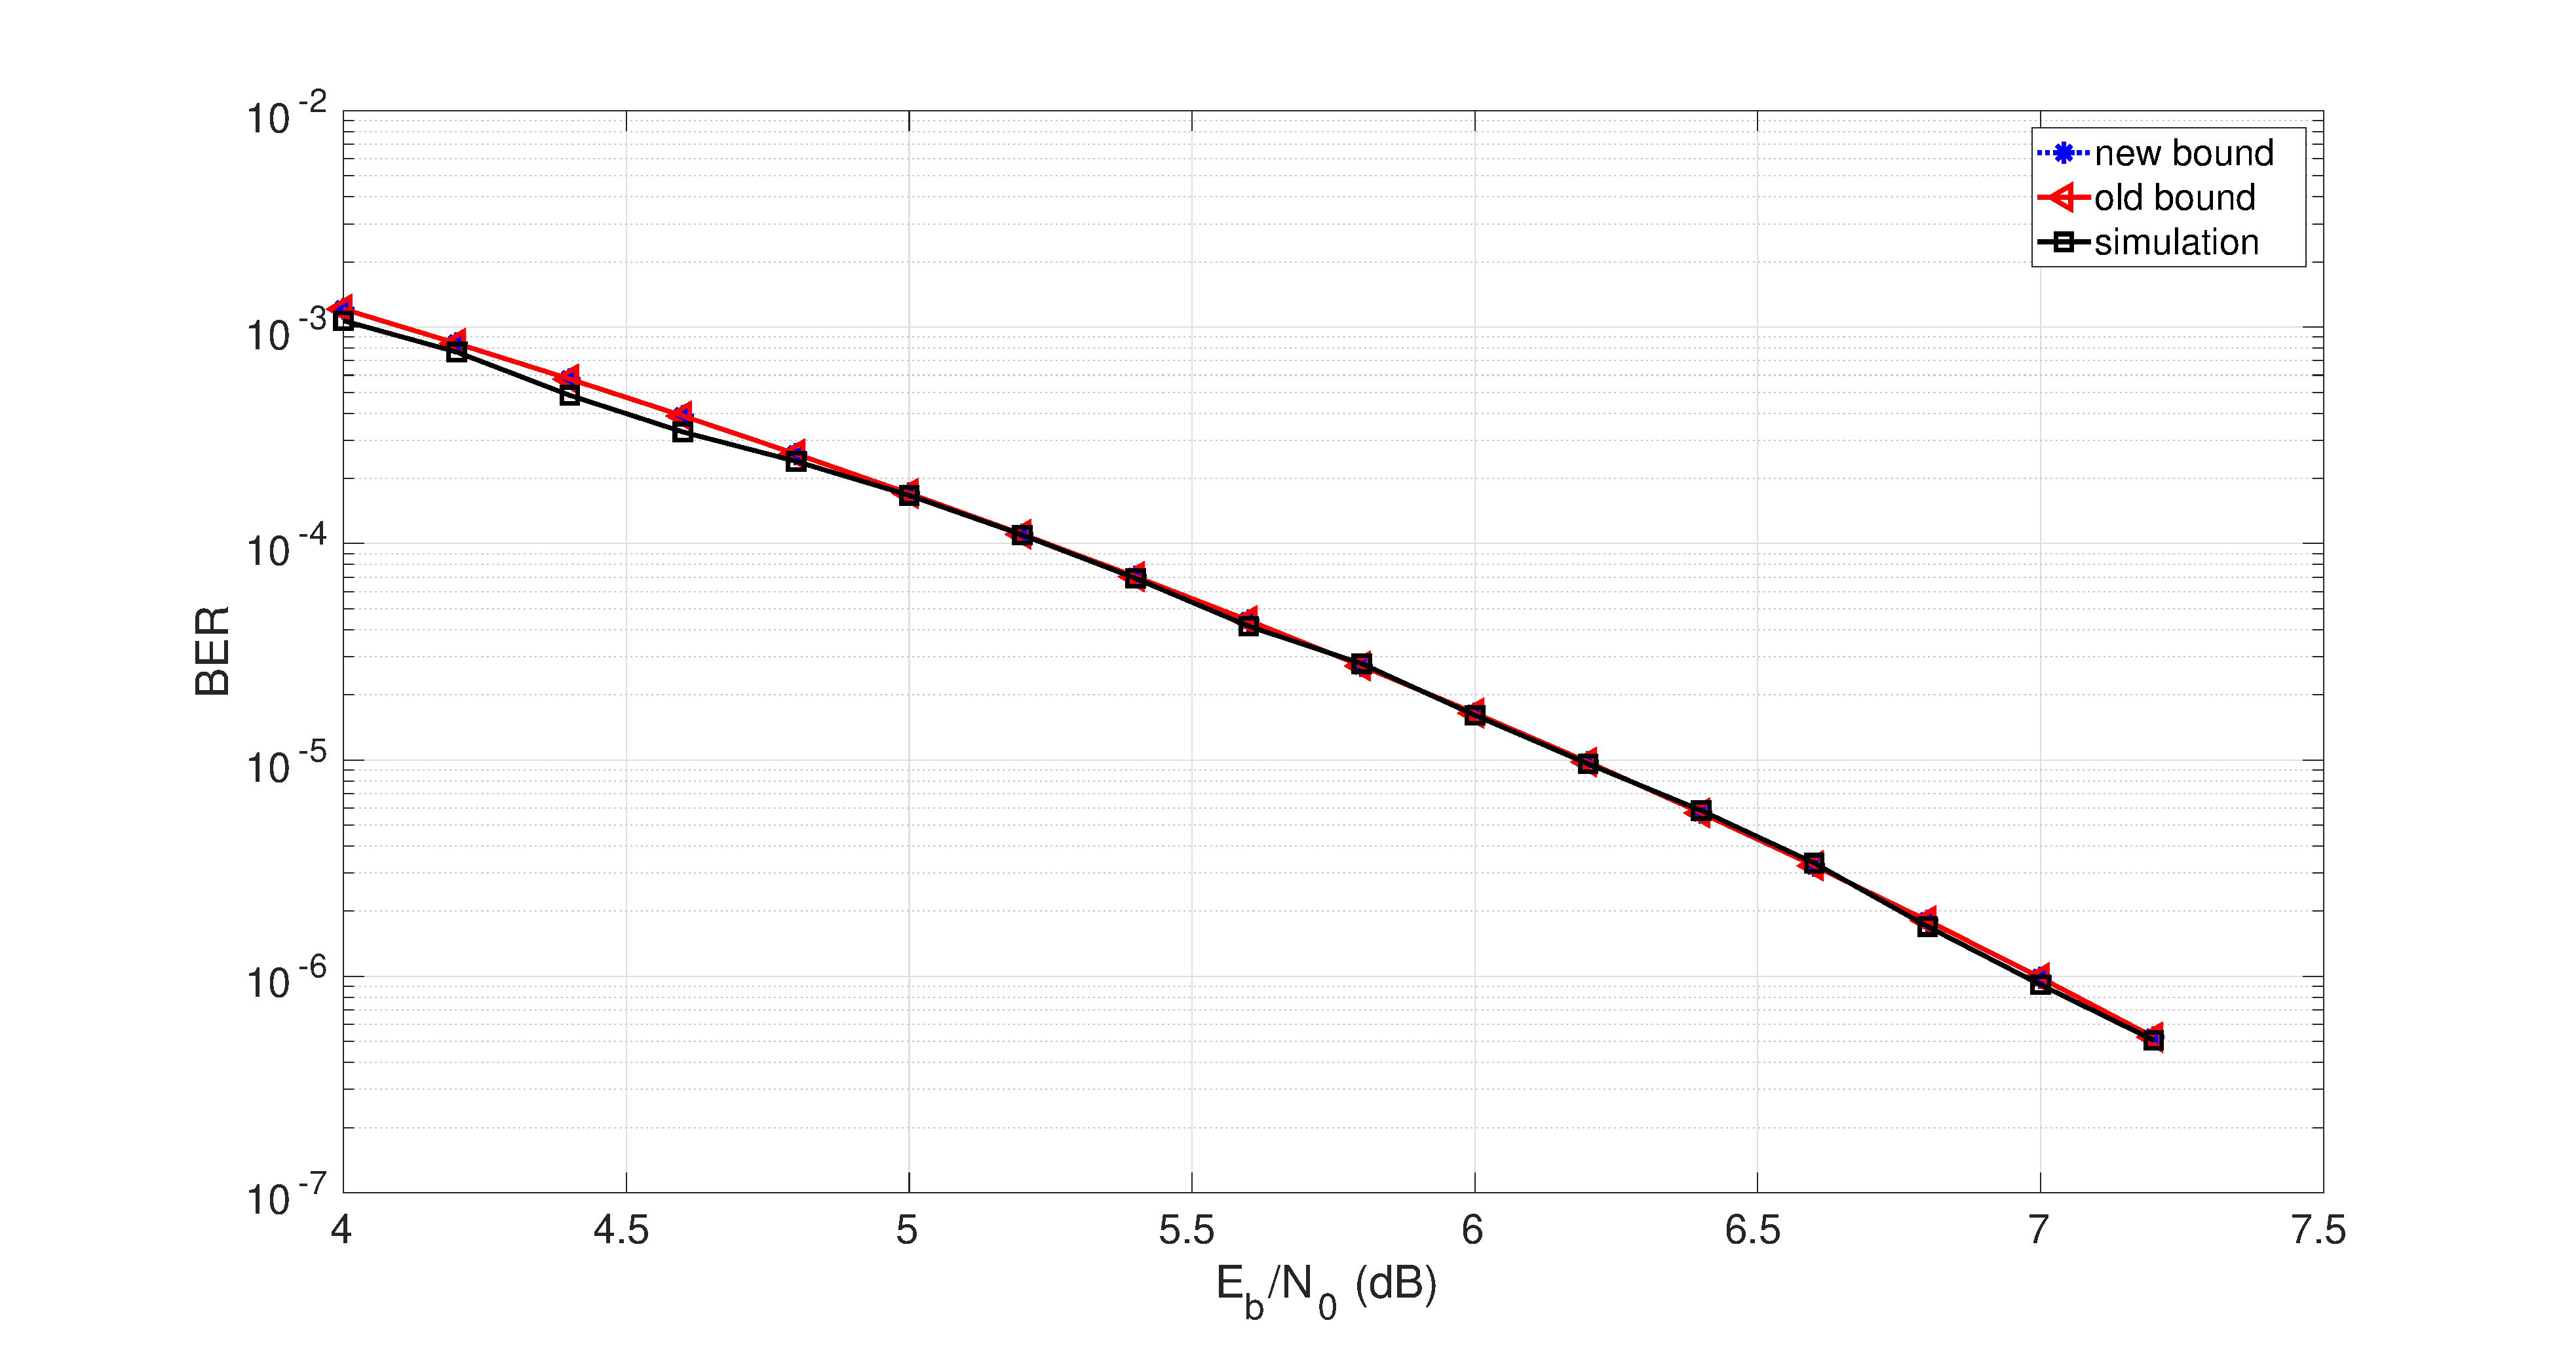
\includegraphics[width=0.8\textwidth]{./Images/RSC_5_7_higher_weights.eps}
%		\caption{Old Bound vs New Bound vs Simulation for 5/7 RSC Code, with higher weights }
%		\label{simFig4}
%		\end{figure}


%		\begin{figure}[h!]
%\centering
%	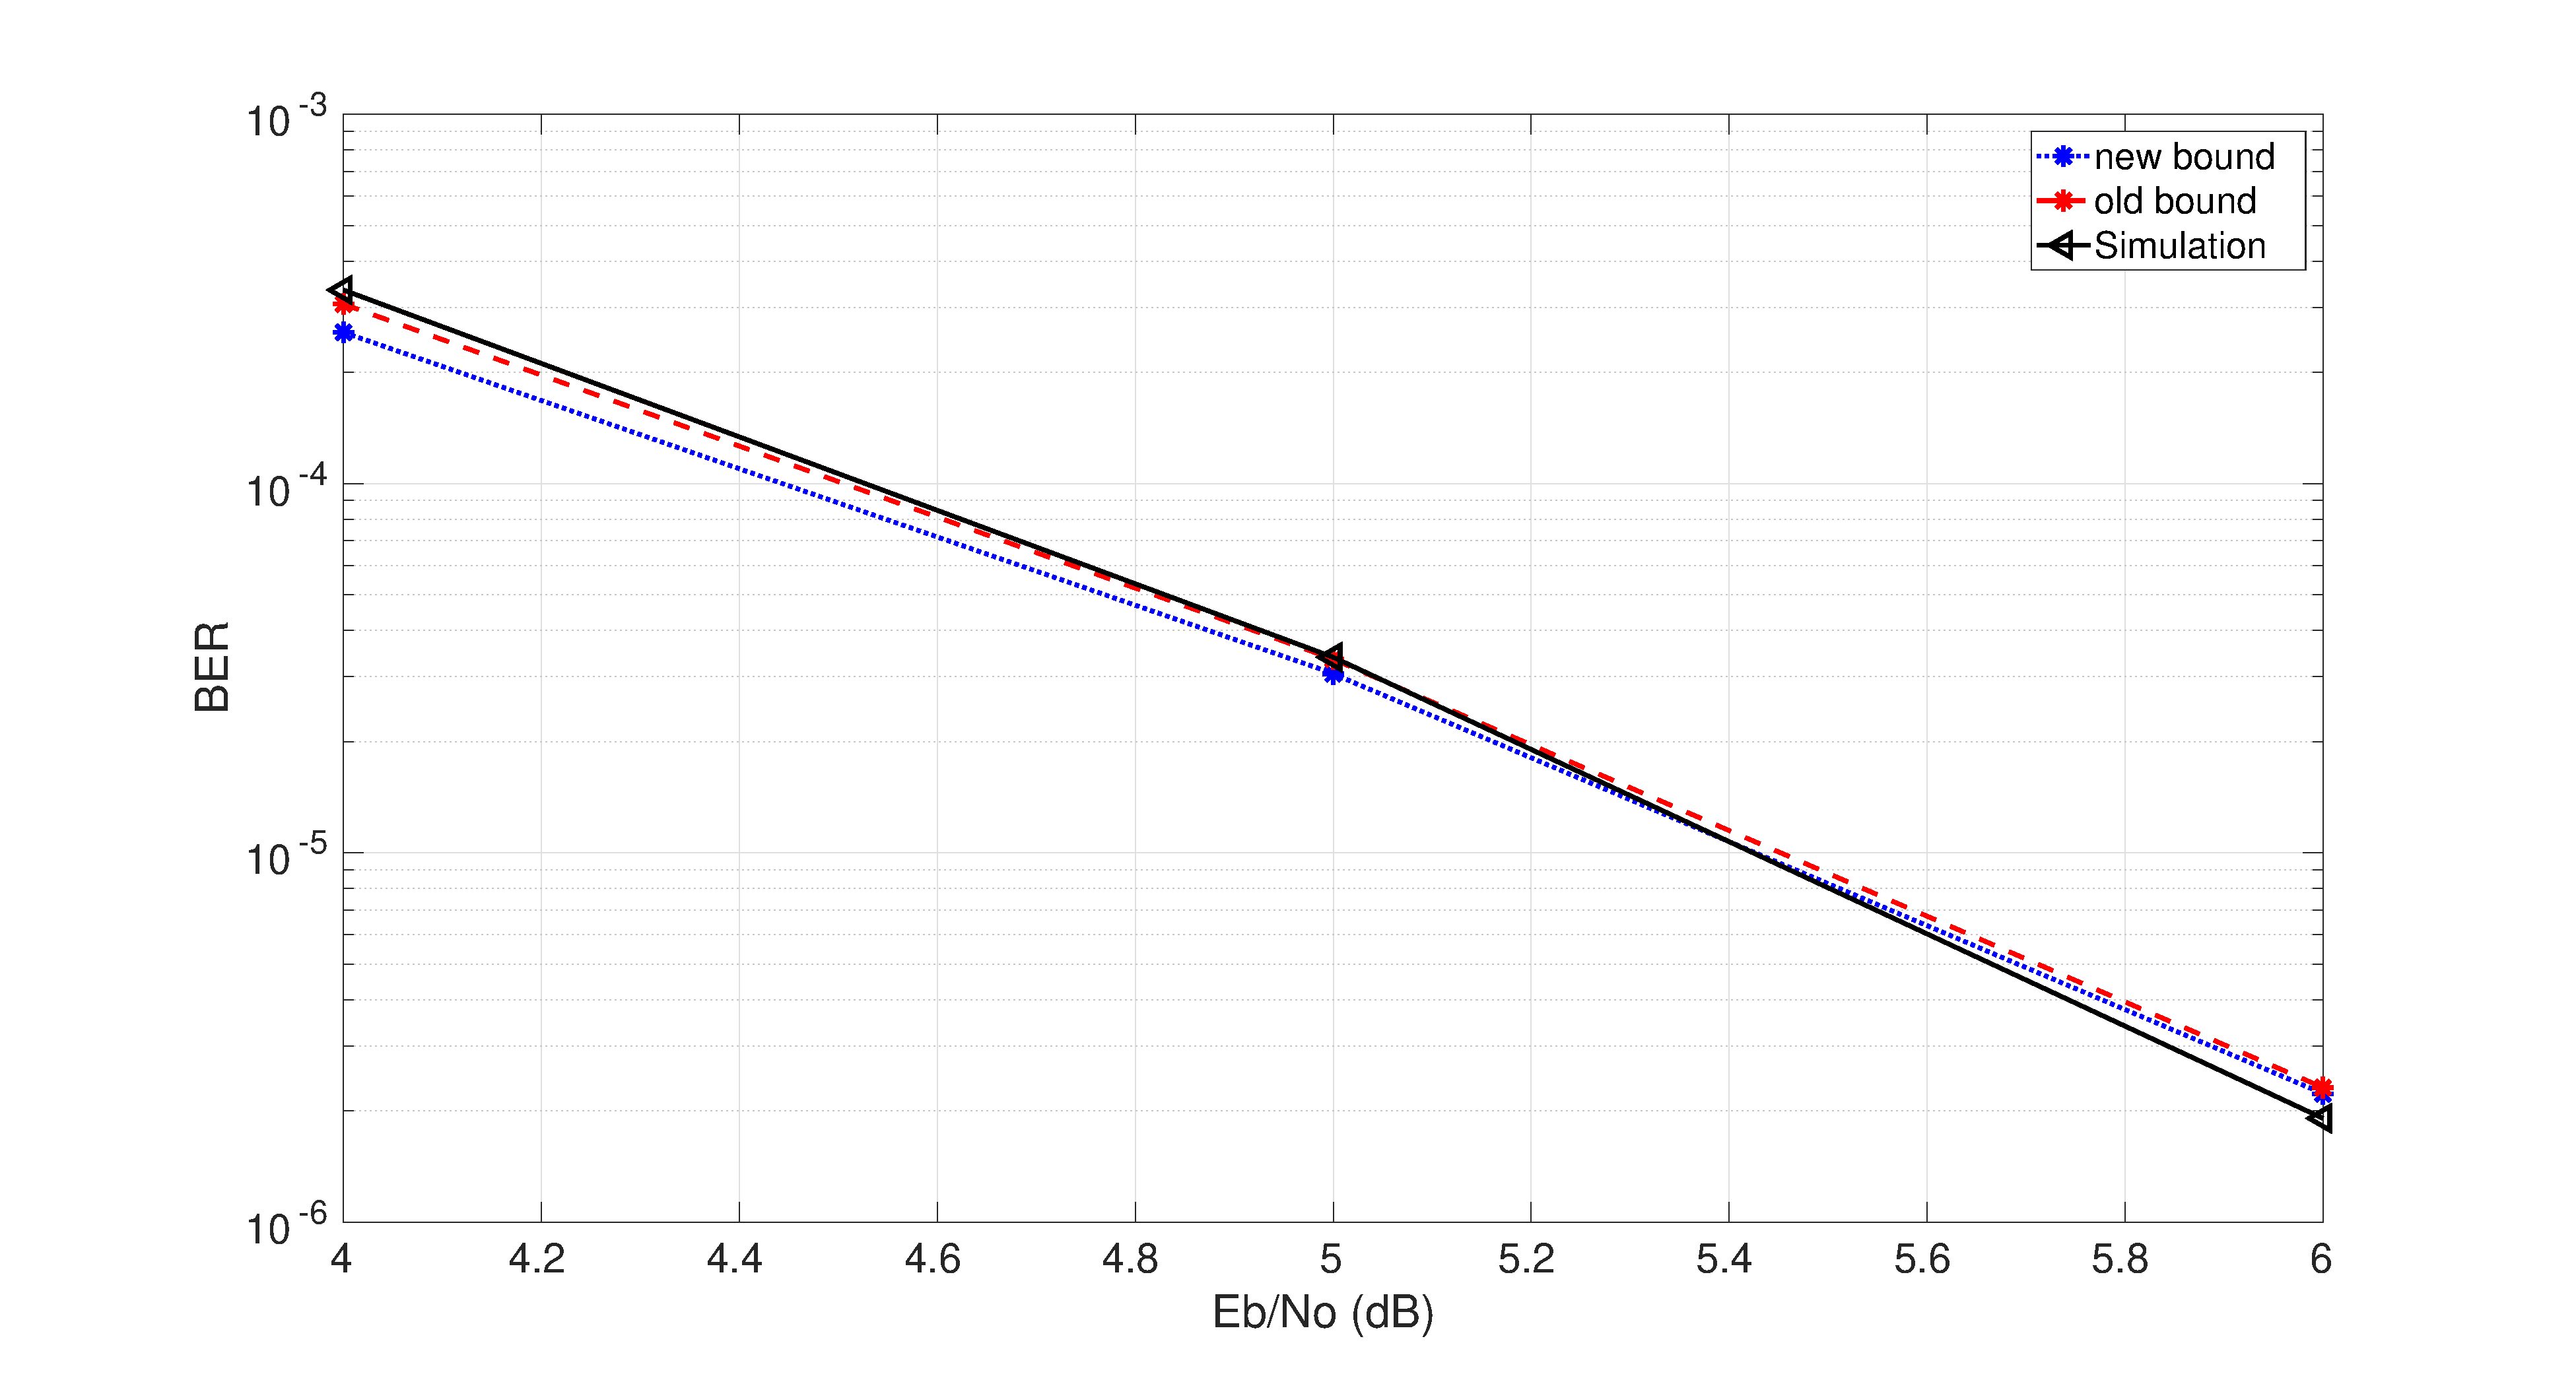
\includegraphics[width=0.5\textwidth]{./Images/RSC_37_21_v2.eps}
%\caption{Old Bound vs New Bound vs Simulation for 37/21 RSC Code, with higher weights}
%\label{simFig5}
%\end{figure}


